\documentclass[conference]{IEEEtran}
\usepackage{cite}
\usepackage{amsmath,amssymb,amsfonts}
\usepackage{graphicx}
\usepackage{textcomp}
\usepackage{xcolor}
\usepackage{url}
\usepackage[hidelinks]{hyperref}
\graphicspath{{results/results/main/analysis/test/figures/}{results/results/dataset/figures/}}

\begin{document}

\title{INT8 Post-Training Quantization and Object Size in Aerial Object Detection}

\author{
\IEEEauthorblockN{Ali Reza Hussaini}
\IEEEauthorblockA{\textit{Department of Computer Science}\\
\textit{Blekinge Institute of Technology (BTH)}\\
Karlskrona, Sweden\\
alhu22@student.bth.se}
\and
\IEEEauthorblockN{Mhd Malek Kisanieh}
\IEEEauthorblockA{\textit{Department of Computer Science}\\
\textit{Blekinge Institute of Technology (BTH)}\\
Karlskrona, Sweden\\
mhki22@student.bth.se}
}

\maketitle

% =========================================================================== ABSTRACT
\begin{abstract}
INT8 post-training quantization is a common way to make object detectors fast enough for
on-board use in drones, and its accuracy cost is usually reported as one aggregate value.
Aerial images, however, are dominated by small objects, which are often assumed to be more
sensitive to reduced numerical precision. This study tests that assumption with a
pre-registered experiment. A YOLOv8n detector was fine-tuned on VisDrone2019-DET and
converted with TensorRT into FP32, FP16 and INT8 engines, using three different INT8 calibration
sets. All engines were evaluated on the same 1,610 test-dev images, and the difference in
relative average precision loss between small and non-small objects was estimated with a paired
image-level bootstrap. INT8 reduced average precision by 6.43 percent for small objects and by
5.47 percent for non-small objects. The difference of 0.96 percentage points had a 95 percent
confidence interval from minus 0.81 to plus 3.03 points. Because the interval includes zero, the
pre-registered result is inconclusive, and the data do not show that INT8 harms small objects
more than larger ones. The difference was positive for all three calibration sets, but none of
the intervals excluded zero. The data rule out a size-dependent penalty larger than about three
percentage points, which is moderate compared with the overall INT8 loss of 5.4 percent.
\end{abstract}

\begin{IEEEkeywords}
aerial imagery, bootstrap, INT8, object detection, post-training quantization, small objects,
TensorRT
\end{IEEEkeywords}

% =========================================================================== INTRODUCTION
\section{Introduction}
\label{sec:introduction}

Unmanned aerial vehicles (UAVs) increasingly run object detectors on board, where memory,
energy and latency budgets are tight. A standard way to meet such budgets is post-training
quantization (PTQ) to 8-bit integers (INT8). A network trained in 32-bit floating point (FP32)
is converted after training, using a small set of calibration images to estimate the value
ranges of its activations; no retraining is
needed~\cite{jacob2018quantization,nagel2021whitepaper}. Deployment toolchains such as TensorRT
make this conversion a routine export step for YOLO
detectors~\cite{ultralytics_tensorrt}. Its accuracy cost is typically reported as a single change
in mean average precision (mAP).

A single overall accuracy score can hide how quantization affects different groups of objects differently. In image classification, compressed networks lose
accuracy disproportionately on a subset of examples rather than uniformly across
them~\cite{hooker2019forget}. In aerial detection, the subset of concern is small objects. They
make up most annotations in drone benchmarks such as
VisDrone~\cite{zhu2022visdrone,cao2021visdrone} and are already the hardest to
detect~\cite{akyon2022sahi}. Two mechanisms make a larger INT8 penalty for small objects
plausible. First, a small object is represented by few activations, and their resolution can
suffer when the quantization range is dominated by large outlier values, a known difficulty of
PTQ for detectors~\cite{nagel2021whitepaper,kim2026inlier}. Second, a localization error of a
single pixel lowers the intersection over union (IoU) of a small box much more than that of a
large box.

If small objects do lose more, aggregate mAP overstates how suitable INT8 is for aerial
deployment, where small objects often matter most. If they do not, size-specific countermeasures
are unnecessary. Detection benchmarks commonly report accuracy by COCO size
group~\cite{lin2014coco}. However, the PTQ studies cited here focus on proposing methods rather
than on testing whether the loss depends on object size. The question addressed here is therefore
the following.

\textbf{Research question:} \emph{In aerial imagery, is the relative loss in detection
accuracy caused by INT8 post-training quantization of a lightweight YOLO detector larger for
small objects than for larger objects?}

The independent variable is numerical precision: an FP32 baseline versus an INT8 treatment, with
an FP16 control. Object size (small vs.\ non-small) is an observed moderator, and the dependent
variable is AP@[.5:.95] per size group. With $D$ defined in Section~\ref{sec:method} as the
relative AP loss of small objects minus that of non-small objects, the hypotheses are
$H_0\!: D\le 0$ and $H_1\!: D>0$.

The study is deliberately narrow: one detector, one dataset and one quantization toolchain, so
that numerical precision is the only manipulated factor. Its contributions are (i) a
pre-registered, paired experimental design in which all precision conditions derive from one
frozen checkpoint and are evaluated on identical images, (ii) a paired image-level bootstrap for
COCO-style AP by object size, and (iii) an estimate, with its uncertainty, of the size-dependence
of INT8 PTQ loss on VisDrone2019-DET. Section~\ref{sec:related-work} reviews related work,
Section~\ref{sec:method} describes the method, Section~\ref{sec:results} reports the results, and
Sections~\ref{sec:discussion} and~\ref{sec:conclusion} discuss and conclude.

% =========================================================================== RELATED WORK
\section{Related Work}
\label{sec:related-work}

\emph{Quantization.} Integer-arithmetic inference with affine quantization of weights and
activations was formalized by Jacob et al.~\cite{jacob2018quantization}. Practical PTQ, including
per-channel weight quantization and calibration of activation ranges, is reviewed by Nagel et
al.~\cite{nagel2021whitepaper} and Krishnamoorthi~\cite{krishnamoorthi2018quantizing}. Wu et
al.~\cite{wu2020integer} compare INT8 calibration methods, including the max-based calibration
used here, and show that INT8 accuracy can be kept within 1\% of FP32 for all networks studied;
as in most PTQ work, accuracy is reported as one aggregate metric per model. Low precision can also be used during training, as in unified
INT8 training by Zhu et al.~\cite{zhu2020int8}. Such approaches change the trained model and are
outside the scope of this study.

\emph{Quantization of detectors.} Kim et al.~\cite{kim2026inlier} study PTQ specifically for
object detection models and address the influence of outlier activations on calibration. Like
most work in this area, they propose a quantization method. The present study instead measures
the behaviour of a standard deployment toolchain~\cite{ultralytics_tensorrt}.

\emph{Small objects in aerial imagery.} VisDrone~\cite{zhu2022visdrone} is a widely used benchmark
for detection in drone imagery, and the VisDrone-DET2021 challenge results~\cite{cao2021visdrone}
document how difficult small, densely packed objects remain. Akyon et al.~\cite{akyon2022sahi}
address small objects through slicing-aided inference, which highlights the role of object scale.
The COCO small/medium/large definition~\cite{lin2014coco} is the standard way to report accuracy
by size.

\emph{Non-uniform effects of compression.} Hooker et al.~\cite{hooker2019forget} showed that
pruned and quantized classifiers lose accuracy disproportionately on a subset of examples. Whether
an analogous, size-related subset exists for detection under INT8 PTQ in aerial imagery is the
question investigated here.

% =========================================================================== METHOD
\section{Method}
\label{sec:method}

\subsection{Study Design}
This study examines whether INT8 post-training quantization causes a larger relative
detection-accuracy loss for small objects than for larger objects in aerial imagery. Precision is
the experimental factor, with a TensorRT FP32 engine as the baseline, an INT8 engine as the
primary treatment, and an FP16 engine as a control. The FP16 control is needed because the
toolchain runs the non-quantized layers of the INT8 engine in FP16. Object size is an observed
moderator. The comparison is paired: all precision conditions are evaluated on the same images.
The design, metrics, size groups and analysis were fixed in a pre-registration dated 7 Oct.\
2026, before any model was trained. It is published with the code and a deviation
log~\cite{hussaini2026researchmethodology}.

For each object-size group $g$, relative AP loss is defined as
\begin{equation}
\mathrm{RelDrop}_{g} =
\frac{\mathrm{AP}^{\mathrm{FP32}}_{g} - \mathrm{AP}^{\mathrm{INT8}}_{g}}
{\mathrm{AP}^{\mathrm{FP32}}_{g}}.
\label{eq:relative-ap-drop}
\end{equation}
The primary contrast is
\begin{equation}
D = \mathrm{RelDrop}_{\mathrm{small}} - \mathrm{RelDrop}_{\mathrm{non\text{-}small}}.
\label{eq:size-interaction}
\end{equation}
The alternative hypothesis is $D>0$, a greater relative quantization loss for small objects. The
null hypothesis is $D\leq 0$. The relative loss is used because small objects start from a much
lower AP. The same proportional harm therefore produces a smaller absolute drop, which would bias
an absolute comparison against the alternative hypothesis.

\subsection{Dataset and Annotation Processing}
The experiment uses VisDrone2019-DET~\cite{zhu2022visdrone}. The training split is used for
fine-tuning and INT8 calibration, the validation split for checkpoint selection and development,
and test-dev only for the final evaluation. The splits contain 6,471 training, 548 validation and
1,610 test-dev images. Dataset archives are verified by SHA-256 before processing.

Annotations are converted to YOLO format for training and to COCO JSON for evaluation. VisDrone
annotations with score zero, which comprise the ignored regions and the ``others'' category, are
excluded. Bounding boxes are clipped to the image boundaries, and boxes with a width or height
below one pixel after clipping are discarded. Detections on excluded ignored regions are therefore treated as
false positives for every condition. As a result, absolute AP values are not directly comparable
with the official VisDrone evaluation toolkit~\cite{cao2021visdrone}, although the paired
comparison is unaffected.

Object size is the area of the clipped ground-truth box in original image pixels. Following the
COCO convention~\cite{lin2014coco}, small objects have an area below $32^2=1{,}024$ pixels and
non-small objects an area of at least $1{,}024$ pixels. The secondary groups are medium
($32^2 \leq \mathrm{area} < 96^2$) and large ($\mathrm{area} \geq 96^2=9{,}216$ pixels).
After processing, test-dev contains 75,102 objects, of which 67.7\% are small, 29.1\% medium and
3.2\% large (60.5\%, 34.0\% and 5.5\% in the training split). Size and class are related:
pedestrians, people and motors make up 58.5\% of small but only 14.4\% of non-small objects,
whereas cars, vans, trucks and buses make up 38.3\% and 82.1\%, respectively.
Size-specific evaluation follows the COCO rule: ground truths outside a size range, detections
matched to them, and unmatched detections outside the range are ignored for that range. Unlike
slicing-aided approaches~\cite{akyon2022sahi}, every precision condition uses the same full-image
input; tiling is not part of the study.

\subsection{Model Training and Engine Construction}
The detector is YOLOv8n~\cite{jocher2023yolov8}, the smallest YOLOv8 variant and a typical
choice for embedded hardware, initialized from COCO-pretrained weights. One model is fine-tuned on the
training split at $640 \times 640$ for 100 epochs, with batch size 16, random seed 0 and
deterministic training. Other options use the Ultralytics defaults, and no hyper-parameter search
is performed. The best checkpoint on the validation split is frozen and used to build all
precision variants.

The frozen checkpoint is exported to ONNX with a static input of $1 \times 3 \times 640 \times
640$ and converted to TensorRT engines with the documented Ultralytics export
workflow~\cite{ultralytics_tensorrt}. The exported ONNX graph is identical for all conditions
(verified by hash) before the precision-specific conversion. Engines are built in FP32, FP16 and
INT8. Three independent INT8 calibration sets are
sampled, one per seed (0, 1 and 2), each consisting of 512 training images drawn uniformly at
random. Calibration and evaluation use the same $640 \times 640$ letterbox preprocessing. The
primary INT8 comparison uses calibration seed 0, and seeds 1 and 2 serve as robustness checks.
For INT8, NVIDIA ModelOpt inserts explicit quantize/dequantize nodes with max calibration, and
layers that are not quantized run in FP16.

\subsection{Evaluation Measures}
The frozen PyTorch checkpoint and every TensorRT engine are evaluated with identical inference
settings: confidence threshold 0.001, non-maximum suppression (NMS) IoU threshold 0.7, at most
500 detections per image, batch size 1, and square $640 \times 640$ input. The primary accuracy
measure is COCO-style AP averaged over IoU thresholds from 0.50 to 0.95 (AP@[.5:.95]); AP at IoU
0.50 (AP@0.5) is secondary. Evaluation is reported overall and by size group.

Predictions are matched to ground truth with pycocotools, and the per-image match records are
stored for the bootstrap. The implementation's AP recomputation must agree with pycocotools to
within $10^{-9}$. As further implementation checks, the PyTorch FP32 checkpoint is compared with
the TensorRT FP32 engine, and the results are compared with Ultralytics' validation metrics. All
development and debugging used the validation split. Each engine was evaluated on test-dev
exactly once (12 Oct.\ 2026), after all engines had been built and evaluated on the validation
split. The confirmatory comparison is TensorRT FP32 versus INT8
calibration seed 0 on test-dev.

\subsection{Statistical Analysis}
AP is computed from detections ranked across the whole test set, so there are no independent
per-image AP values for a classical paired test. A paired nonparametric
bootstrap~\cite{efron1993bootstrap} is therefore used, with the image as the resampling unit. It
draws 2,000 resamples of the 1,610 test-dev images with replacement (random seed 0). The same
resampled image indices are used for every precision condition and contrast, which preserves the
pairing. For each resample, AP is recomputed by size group from the stored match records, without
re-matching detections.

The confirmatory statistic is $D$ in~\eqref{eq:size-interaction} for FP32 versus INT8 seed 0 on
AP@[.5:.95], with a two-sided 95\% percentile bootstrap confidence interval. If the lower bound is
above zero, the null hypothesis is rejected in favour of a greater relative loss for small
objects. If the interval contains zero, the result is inconclusive, and if the upper bound is
below zero, the result is contrary to the alternative hypothesis. Because $H_1$ is directional,
this rule corresponds to a one-sided test at $\alpha=0.025$.

The percentile bootstrap makes no normality assumption about $D$, which is a ratio-based
quantity with an unknown sampling distribution. It does assume that test images are independent
and that the resampled AP is well defined. Both are checked: AP must be finite for every
resample, the shape of the bootstrap distribution is inspected for skew and bias, and possible
dependence between images of the same scene is discussed as a validity threat. The image is
used as the unit because VisDrone test-dev file names do not reliably identify video sequences,
so no sound cluster structure was available. This was decided from the labels alone, before any
model output was produced.

All other comparisons are exploratory and are reported with confidence intervals only. These are
absolute AP drops, AP@0.5, small/medium/large AP, calibration seeds 1 and 2, and the FP16 control.
The INT8 result is considered directionally robust if $D$ has the same sign for all three
calibration seeds. The FP16 control shows whether a size-dependent effect is specific to INT8: a
similar pattern under FP16 would prevent attributing it to INT8 alone. Exploratory intervals are
not adjusted for multiplicity and are therefore not used for hypothesis testing. The implementation of
training, conversion, evaluation and analysis is available in the project
repository~\cite{hussaini2026researchmethodology}.

\subsection{Experimental Setup and Deviations}
All main-study training, engine builds and evaluations ran on one NVIDIA GeForce RTX 5080 (16\,GB) in one
fixed environment: Python 3.11.9, PyTorch 2.10.0+cu128, Ultralytics 8.4.174 and TensorRT
11.3.0.99. Ultralytics and TensorRT match the pre-registration. Python and PyTorch differ from
the versions in the project's setup instructions (3.12 and 2.14.1); every run log from the first
training onward shows the versions actually used. The pre-registered latency benchmark, a
secondary outcome, was not implemented. As the pre-registered fallback allows, only the
per-image inference times recorded by Ultralytics during evaluation are reported. Both
deviations are listed in the deviation log of the pre-registration, which was completed after
the experiment. Neither affects the confirmatory analysis.

The study uses only a public benchmark released for research~\cite{zhu2022visdrone}. It involves
no human participants, and no images are redistributed or used to identify people.

% =========================================================================== RESULTS
\section{Results}
\label{sec:results}

\subsection{Test-Set Detection Accuracy}
The final evaluation covered 1,610 test-dev images containing 75,102 retained ground-truth
objects. Table~\ref{tab:ap-results} reports AP@[.5:.95] overall and for all size groups shown in
Fig.~\ref{fig:ap-size}; the non-small group is the union of the medium and large groups. Values
are on a 0--100 scale, and confidence intervals are 95\% paired image-bootstrap percentile
intervals. INT8 seed 0 had lower point estimates than FP32 in every group. In absolute terms, INT8
lost 0.43 AP points for small objects and 1.39 points for non-small objects.


\begin{table}[!t]
\caption{Test-dev AP@[.5:.95] by object-size group. Point estimates with 95\% paired-bootstrap
confidence intervals, on a 0--100 scale.}
\label{tab:ap-results}
\centering
\footnotesize
\setlength{\tabcolsep}{4pt}
\begin{tabular}{lrll}
\hline
Group & Objects & FP32 & INT8 seed 0 \\
\hline
Small     & 50,816 & 6.62 [6.22, 7.19]    & 6.19 [5.83, 6.72] \\
Non-small & 24,286 & 25.32 [24.56, 26.49] & 23.93 [23.21, 25.05] \\
Medium    & 21,876 & 23.93 [23.19, 25.08] & 22.58 [21.87, 23.68] \\
Large     & 2,410  & 35.84 [32.57, 42.52] & 33.57 [30.59, 40.63] \\
All       & 75,102 & 15.44 [14.88, 16.15] & 14.60 [14.06, 15.28] \\
\hline
\end{tabular}
\end{table}

\begin{figure}[!t]
\centering
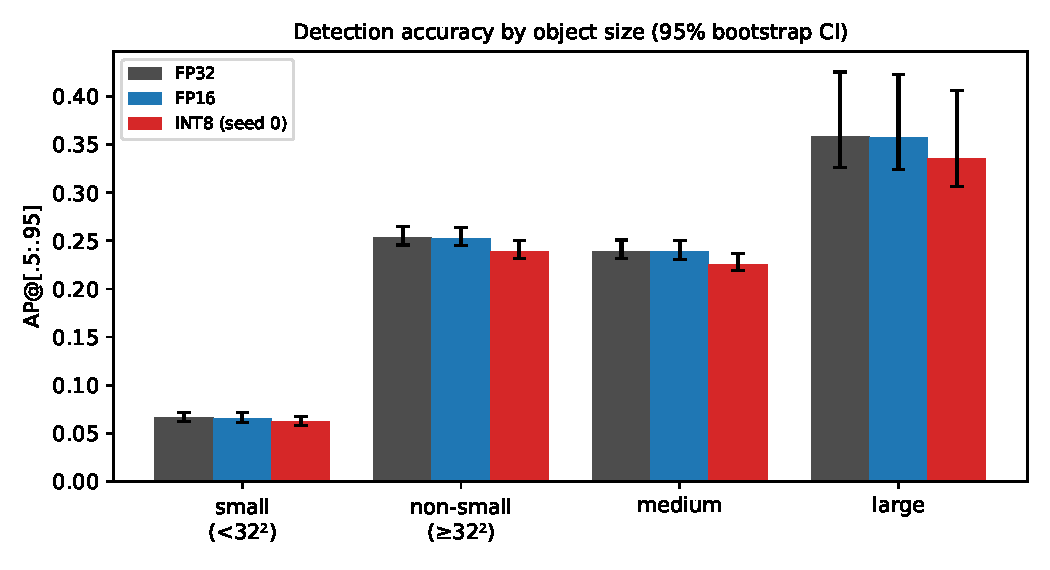
\includegraphics[width=\columnwidth]{fig2_ap_by_size_AP50_95.pdf}
\caption{Test-dev AP@[.5:.95] (0--1 scale) by object-size group for FP32, FP16 and INT8 seed 0.
Error bars show 95\% paired-bootstrap confidence intervals.}
\label{fig:ap-size}
\end{figure}

\subsection{Confirmatory Size-Dependent Loss}
For INT8 seed 0, the relative AP loss was 6.43\% for small objects and 5.47\% for non-small
objects (Fig.~\ref{fig:relative-loss}). Their difference was $D=+0.96$ percentage points, with a
95\% confidence interval of $[-0.81,\,+3.03]$ percentage points. Because the interval contains
zero, the pre-registered result is inconclusive and does not support the hypothesis that INT8
causes a larger relative AP loss for small objects. Fig.~\ref{fig:d-bootstrap} shows the
bootstrap distribution of the primary contrast.

\begin{figure}[!t]
\centering
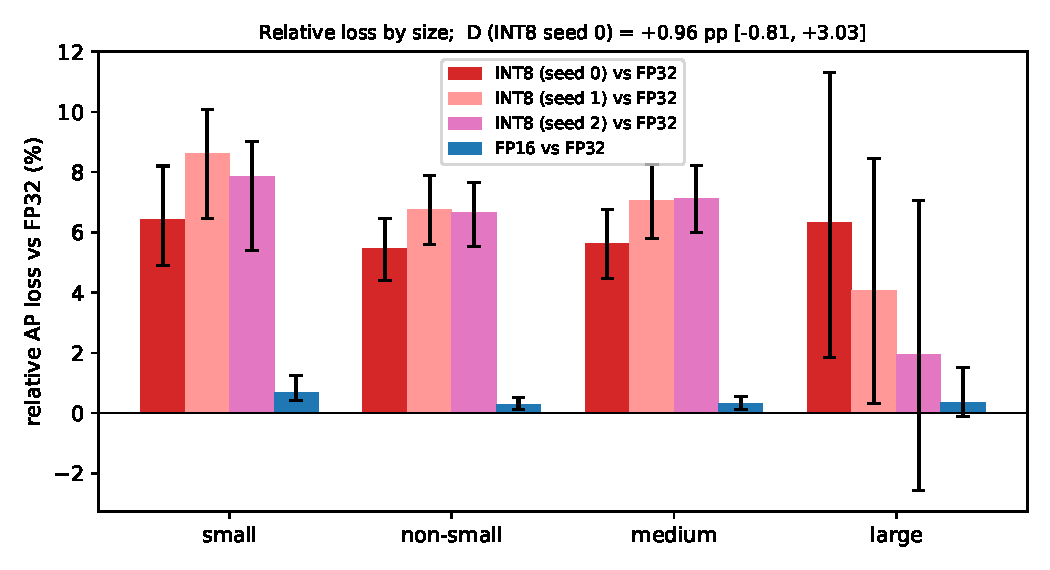
\includegraphics[width=\columnwidth]{fig3_relative_drop_AP50_95.pdf}
\caption{Relative AP@[.5:.95] loss versus FP32 by object-size group for the three INT8
calibration seeds and FP16. Error bars show 95\% paired-bootstrap confidence intervals. The
primary comparison is INT8 seed 0 versus FP32.}
\label{fig:relative-loss}
\end{figure}

\begin{figure}[!t]
\centering
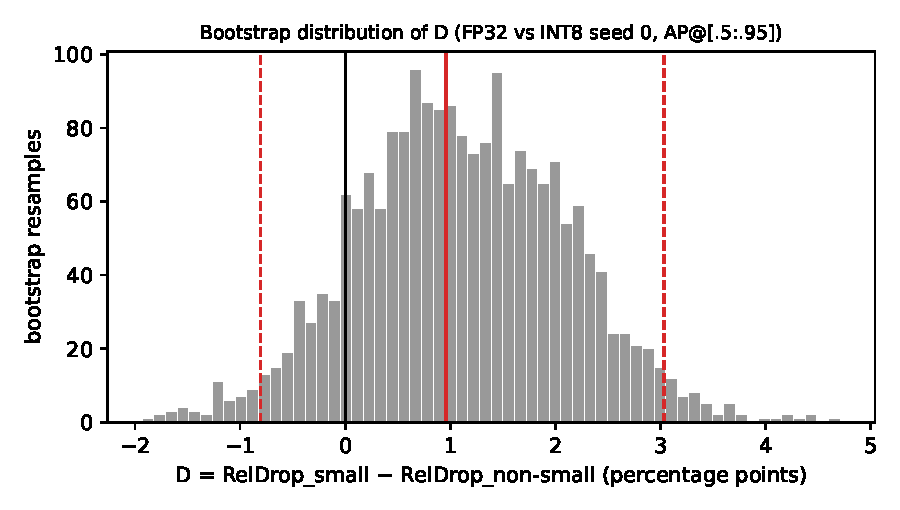
\includegraphics[width=\columnwidth]{figA_D_bootstrap.pdf}
\caption{Paired-bootstrap distribution of $D$ for the primary FP32 versus INT8 seed 0 comparison.
The solid line marks the point estimate, the dashed lines the 95\% confidence limits, and the zero
line no difference in relative loss by size.}
\label{fig:d-bootstrap}
\end{figure}

\begin{table}[!t]
\caption{Relative AP loss versus TensorRT FP32 (\%), the size contrast $D$ and its absolute
counterpart $D_{\mathrm{abs}}$ (AP points), with 95\% paired-bootstrap confidence intervals, on
AP@[.5:.95] unless marked AP50. The first row is the confirmatory test; all other rows are
exploratory.}
\label{tab:contrasts}
\centering
\scriptsize
\setlength{\tabcolsep}{2pt}
\begin{tabular}{lrrll}
\hline
Condition & Small & Non-s. & $D$ [95\% CI] & $D_{\mathrm{abs}}$ [95\% CI] \\
\hline
INT8 s0          & 6.43 & 5.47 & $+0.96$ [$-0.81$, $+3.03$] & $-0.96$ [$-1.24$, $-0.65$] \\
INT8 s0 (AP50)   & 4.57 & 4.87 & $-0.30$ [$-1.74$, $+1.95$] & $-1.42$ [$-1.87$, $-0.79$] \\
INT8 s1          & 8.60 & 6.77 & $+1.83$ [$-0.60$, $+3.72$] & $-1.14$ [$-1.49$, $-0.84$] \\
INT8 s2          & 7.84 & 6.65 & $+1.19$ [$-1.34$, $+2.66$] & $-1.17$ [$-1.49$, $-0.91$] \\
FP16             & 0.70 & 0.28 & $+0.42$ [$+0.07$, $+0.98$] & $-0.02$ [$-0.08$, $+0.03$] \\
\hline
\end{tabular}
\end{table}

\subsection{Exploratory Comparisons}
Table~\ref{tab:contrasts} summarizes the exploratory contrasts. The point estimate of $D$ was
positive for all three INT8 calibration seeds ($+0.96$, $+1.83$ and $+1.19$ percentage points),
which meets the pre-registered criterion for directional robustness. All three intervals included
zero, however, so the confirmatory finding remains inconclusive. The overall relative loss
varied more between seeds (5.4\%, 7.4\% and 7.0\%) than $D$ did. On AP@0.5, $D$ was close to zero
for every seed. On the absolute scale, $D_{\mathrm{abs}}$ was negative for every seed with
intervals excluding zero: in AP points, small objects lost less than non-small objects.

The FP16 engine lost only 0.37\% of overall AP, which shows that TensorRT conversion itself
costs little accuracy and that the INT8 loss comes from quantization. Its $D$ was $+0.42$
percentage points with an interval just above zero, although $D_{\mathrm{abs}}$ was essentially
zero. Because the primary INT8 interval includes zero, the pre-registered FP16 attribution rule
is not triggered.

\subsection{Assumption and Implementation Checks}
All 2,000 resamples produced finite AP values for every condition and size group. The bootstrap
distribution of $D$ (Fig.~\ref{fig:d-bootstrap}) is unimodal and nearly symmetric (skewness
0.06), with a standard error of 0.99 percentage points. Its mean exceeds the point estimate by
only 0.16 points. A normal-approximation interval (point estimate $\pm1.96$ standard errors,
$[-0.99,\,+2.91]$) also contains zero, so the decision does not depend on the interval method.
The implementation's AP matched pycocotools to within $2\times10^{-16}$ for every engine.
TensorRT FP32 and PyTorch FP32 differed by less than $10^{-4}$ AP@[.5:.95] in every size group,
so the TensorRT FP32 engine is a faithful baseline. Overall AP differed from Ultralytics' own
validator by 0.0028--0.0029 for every TensorRT engine. The offset reflects a different AP implementation; it is
nearly constant across conditions and therefore does not affect the paired contrasts.

\subsection{Latency}
The controlled latency benchmark was not run (Section~\ref{sec:method}). The per-image
inference times that Ultralytics recorded during test-dev evaluation were 0.77\,ms for FP32,
0.42\,ms for FP16 and 0.69--0.71\,ms for the three INT8 engines. These times come from an
uncontrolled protocol and are descriptive only.

% =========================================================================== DISCUSSION
\section{Discussion}
\label{sec:discussion}

The results do not provide sufficient evidence that INT8 post-training quantization causes a
greater relative detection-accuracy loss for small objects than for non-small objects. The
relative loss was higher for small objects (6.43\%) than for non-small objects (5.47\%), but the
difference of 0.96 percentage points had a 95\% confidence interval spanning zero. The primary
hypothesis was therefore not supported. This finding is inconclusive; it is not evidence that the
two groups are affected equally. The interval does, however, bound the effect. A size-dependent
penalty larger than about 3 percentage points, meaning a small-object relative loss above roughly
8.5\% against 5.5\% for non-small objects, is not compatible with the data. Compared with the
overall INT8 loss of 5.4\%, any size-dependent component is therefore at most moderate.

The relative and absolute views point in different directions. Small objects lost proportionally
slightly more, whereas non-small objects lost about three times more AP points (1.39 vs.\ 0.43).
Statements that quantization ``hurts small objects more'' thus depend on the scale used. The
relative scale was pre-registered because the baselines differ by a factor of about four. The
mechanisms proposed in the introduction also act on different scales. Coarser activations would
tend to make small objects disappear, which should show up at IoU 0.5. Localization jitter would
mainly hurt small objects at high IoU thresholds. That $D$ was near zero on AP@0.5 but slightly
positive on AP@[.5:.95] is weakly consistent with the second mechanism rather than the first,
but the difference is well within the uncertainty.

The positive estimates across all three calibration seeds indicate a consistent direction, but
the seeds share the same model and test images and are not independent replications. The choice
of calibration set changed the overall INT8 loss by two percentage points, which is larger than
the size contrast itself. The FP16 control lost almost no accuracy overall, yet produced a small
positive $D$ with an interval just above zero. Because the small-object FP16 loss amounts to only
0.05 AP points, this relative difference is fragile. It may indicate that very small objects are
sensitive to any reduction in precision, or it may be a chance finding among several uncorrected
exploratory intervals. Outlier-sensitive calibration, as studied by Kim et
al.~\cite{kim2026inlier}, is one possible mechanism for differences between calibration sets;
this experiment does not test that mechanism.

\subsection{Threats to Validity}
\emph{Internal validity.} All conditions share one checkpoint, one ONNX graph, identical
preprocessing and identical images, so precision is the only manipulated factor. TensorRT does,
however, choose kernels and layer fusions per precision, and the INT8 engine runs its
unquantized layers in FP16. The FP16 control bounds this toolchain effect but cannot fully
separate it from quantization.

\emph{Construct validity.} Object size is observed, not assigned. Small and non-small objects
differ in class composition (Section~\ref{sec:method}), so $D$ measures size and class together. Small objects also start
from a low AP of 0.066, which makes relative losses noisy. The excluded ignored regions mean that
absolute AP differs from the official VisDrone protocol~\cite{cao2021visdrone}, although the
same rule applies to every condition. Latency was not measured under a controlled protocol. The
recorded times show no speed-up of INT8 over FP16 at batch size 1, so the study cannot show that
the accuracy loss buys faster inference on this GPU.

\emph{Conclusion validity.} The bootstrap captures variation across test images but not variation
from model training or hardware. Correlation between images of the same scene would make its
intervals too narrow, which would make a significant result less trustworthy. It does not explain
the inconclusive one. The CI width of about 4 percentage points means the study could detect
only a moderate size effect. Finally, the pre-registration was not deposited in a time-stamped
registry, and the public repository was first committed after the test-dev analysis. Its date
therefore rests on the authors' own record.

\emph{External validity.} The experiment uses one YOLOv8n model, one dataset and a $640\times640$
full-image input, which downscales the original images. Slicing-aided
inference~\cite{akyon2022sahi} enlarges small objects in the input, so the findings should not
be generalized to tiled pipelines, larger detectors or other quantization toolchains.

% =========================================================================== CONCLUSION
\section{Conclusion}
\label{sec:conclusion}

This study investigated whether INT8 post-training quantization causes a greater relative
detection-accuracy loss for small objects than for non-small objects in aerial imagery. A
fine-tuned YOLOv8n detector was evaluated as TensorRT FP32, FP16 and INT8 engines on the
VisDrone2019-DET test-dev split, using size-specific AP and a paired image-level bootstrap.

For the primary FP32-versus-INT8 comparison, the relative AP loss was 6.43\% for small objects
and 5.47\% for non-small objects. The difference of 0.96 percentage points had a 95\% confidence
interval of $[-0.81,\,+3.03]$ percentage points. Since the interval includes zero, the analysis
did not establish that small objects suffer a greater relative loss. The consistent direction
across three calibration seeds did not resolve this uncertainty. In absolute AP points, small
objects lost significantly less than non-small objects. The FP16 control lost almost no accuracy,
so the overall loss of 5--7\% is caused by INT8 quantization, but the size pattern is not
necessarily specific to INT8.

Overall, the experiment provides no conclusive evidence for a size-dependent INT8 accuracy loss
under the evaluated conditions. Future work should test additional models and datasets, separate
the effects of object size and class, and measure inference performance alongside accuracy to
quantify the practical trade-offs of post-training quantization for aerial object detection.

% =========================================================================== REFERENCES
\begin{thebibliography}{00}

\bibitem{jacob2018quantization}
B. Jacob \textit{et al.}, ``Quantization and training of neural networks for efficient
integer-arithmetic-only inference,'' in \textit{Proc. IEEE/CVF Conf. Comput. Vis. Pattern
Recognit. (CVPR)}, 2018, pp. 2704--2713, doi: 10.1109/CVPR.2018.00286.

\bibitem{nagel2021whitepaper}
M. Nagel, M. Fournarakis, R. A. Amjad, Y. Bondarenko, M. van Baalen, and T. Blankevoort,
``A white paper on neural network quantization,'' arXiv:2106.08295, 2021.

\bibitem{ultralytics_tensorrt}
Ultralytics, ``TensorRT export for YOLO26 models,'' \textit{Ultralytics Documentation}. [Online].
Available: \url{https://docs.ultralytics.com/integrations/tensorrt}. Accessed: Oct. 22, 2026.

\bibitem{hooker2019forget}
S. Hooker, A. Courville, G. Clark, Y. Dauphin, and A. Frome, ``What do compressed deep neural
networks forget?'' arXiv:1911.05248, 2019.

\bibitem{zhu2022visdrone}
P. Zhu \textit{et al.}, ``Detection and tracking meet drones challenge,'' \textit{IEEE Trans.
Pattern Anal. Mach. Intell.}, vol. 44, no. 11, pp. 7380--7399, Nov. 2022,
doi: 10.1109/TPAMI.2021.3119563.

\bibitem{cao2021visdrone}
Y. Cao \textit{et al.}, ``VisDrone-DET2021: The vision meets drone object detection challenge
results,'' in \textit{Proc. IEEE/CVF Int. Conf. Comput. Vis. Workshops (ICCVW)}, 2021,
pp. 2847--2854, doi: 10.1109/ICCVW54120.2021.00319.

\bibitem{akyon2022sahi}
F. C. Akyon, S. O. Altinuc, and A. Temizel, ``Slicing aided hyper inference and fine-tuning for
small object detection,'' in \textit{Proc. IEEE Int. Conf. Image Process. (ICIP)}, 2022,
pp. 966--970, doi: 10.1109/ICIP46576.2022.9897990.

\bibitem{kim2026inlier}
M. Kim, D. Lee, J. Yu, J. Hur, G. Kim, and J. Kim, ``Inlier-centric post-training quantization
for object detection models,'' arXiv:2602.03472, Feb. 2026.

\bibitem{lin2014coco}
T.-Y. Lin \textit{et al.}, ``Microsoft COCO: Common objects in context,'' in \textit{Proc. Eur.
Conf. Comput. Vis. (ECCV)}, 2014, pp. 740--755, doi: 10.1007/978-3-319-10602-1\_48.

\bibitem{krishnamoorthi2018quantizing}
R. Krishnamoorthi, ``Quantizing deep convolutional networks for efficient inference: A
whitepaper,'' arXiv:1806.08342, 2018.

\bibitem{wu2020integer}
H. Wu, P. Judd, X. Zhang, M. Isaev, and P. Micikevicius, ``Integer quantization for deep learning
inference: Principles and empirical evaluation,'' arXiv:2004.09602, 2020.

\bibitem{zhu2020int8}
F. Zhu \textit{et al.}, ``Towards unified INT8 training for convolutional neural network,'' in
\textit{Proc. IEEE/CVF Conf. Comput. Vis. Pattern Recognit. (CVPR)}, 2020, pp. 1966--1976,
doi: 10.1109/CVPR42600.2020.00204.

\bibitem{hussaini2026researchmethodology}
A. R. Hussaini and M. M. Kisanieh, ``ResearchMethodology: Experimental repository,'' GitHub
repository. [Online]. Available: \url{https://github.com/alhu22/ResearchMethodology}.
Accessed: Oct. 22, 2026.

\bibitem{jocher2023yolov8}
G. Jocher, A. Chaurasia, and J. Qiu, ``Ultralytics YOLOv8,'' version 8.0.0, software, 2023.
[Online]. Available: \url{https://github.com/ultralytics/ultralytics}. Accessed: Oct. 22, 2026.

\bibitem{efron1993bootstrap}
B. Efron and R. J. Tibshirani, \textit{An Introduction to the Bootstrap}. New York, NY, USA:
Chapman \& Hall, 1993.

\end{thebibliography}

\end{document}
